\section{Use Cases Model}
\label{sec:Use Cases Model}
% Descirbes the functional requirements, mostly non-functional. During incepeion, the names of most use cases will be indentified, and perhapss 10% of teh use cases will be analyzed in detail.
% 
\subsection{Actors}
\label{subsec:Actors}
\begin{table}[htp]
  \definecolor{tcA}{rgb}{0.862745,0.862745,0.862745}
  \begin{tabular}[t]{|l|l|l|}\hline
  % use packages: color,colortbl
	  \rowcolor{tcA}
	  Actor 		& Typ 		& Beschreibung \\\hline
	  User		 	& primary 	& Interagiert mit dem System. \\\hline
	  Operating System 	& supporting 	& Dient dem System beim Zugriff auf das Dateisystem. \\\hline
	  Algorithm Developer 	& offstage 	& Entwickler von Algorithmen. \\\hline
  \end{tabular}
  \caption{Actors}
  \label{tab:actors}
\end{table}

% 
\subsection{Use Cases Diagram}
\label{subsec:Use Cases Diagram}
\begin{figure}[H]
    \centering
    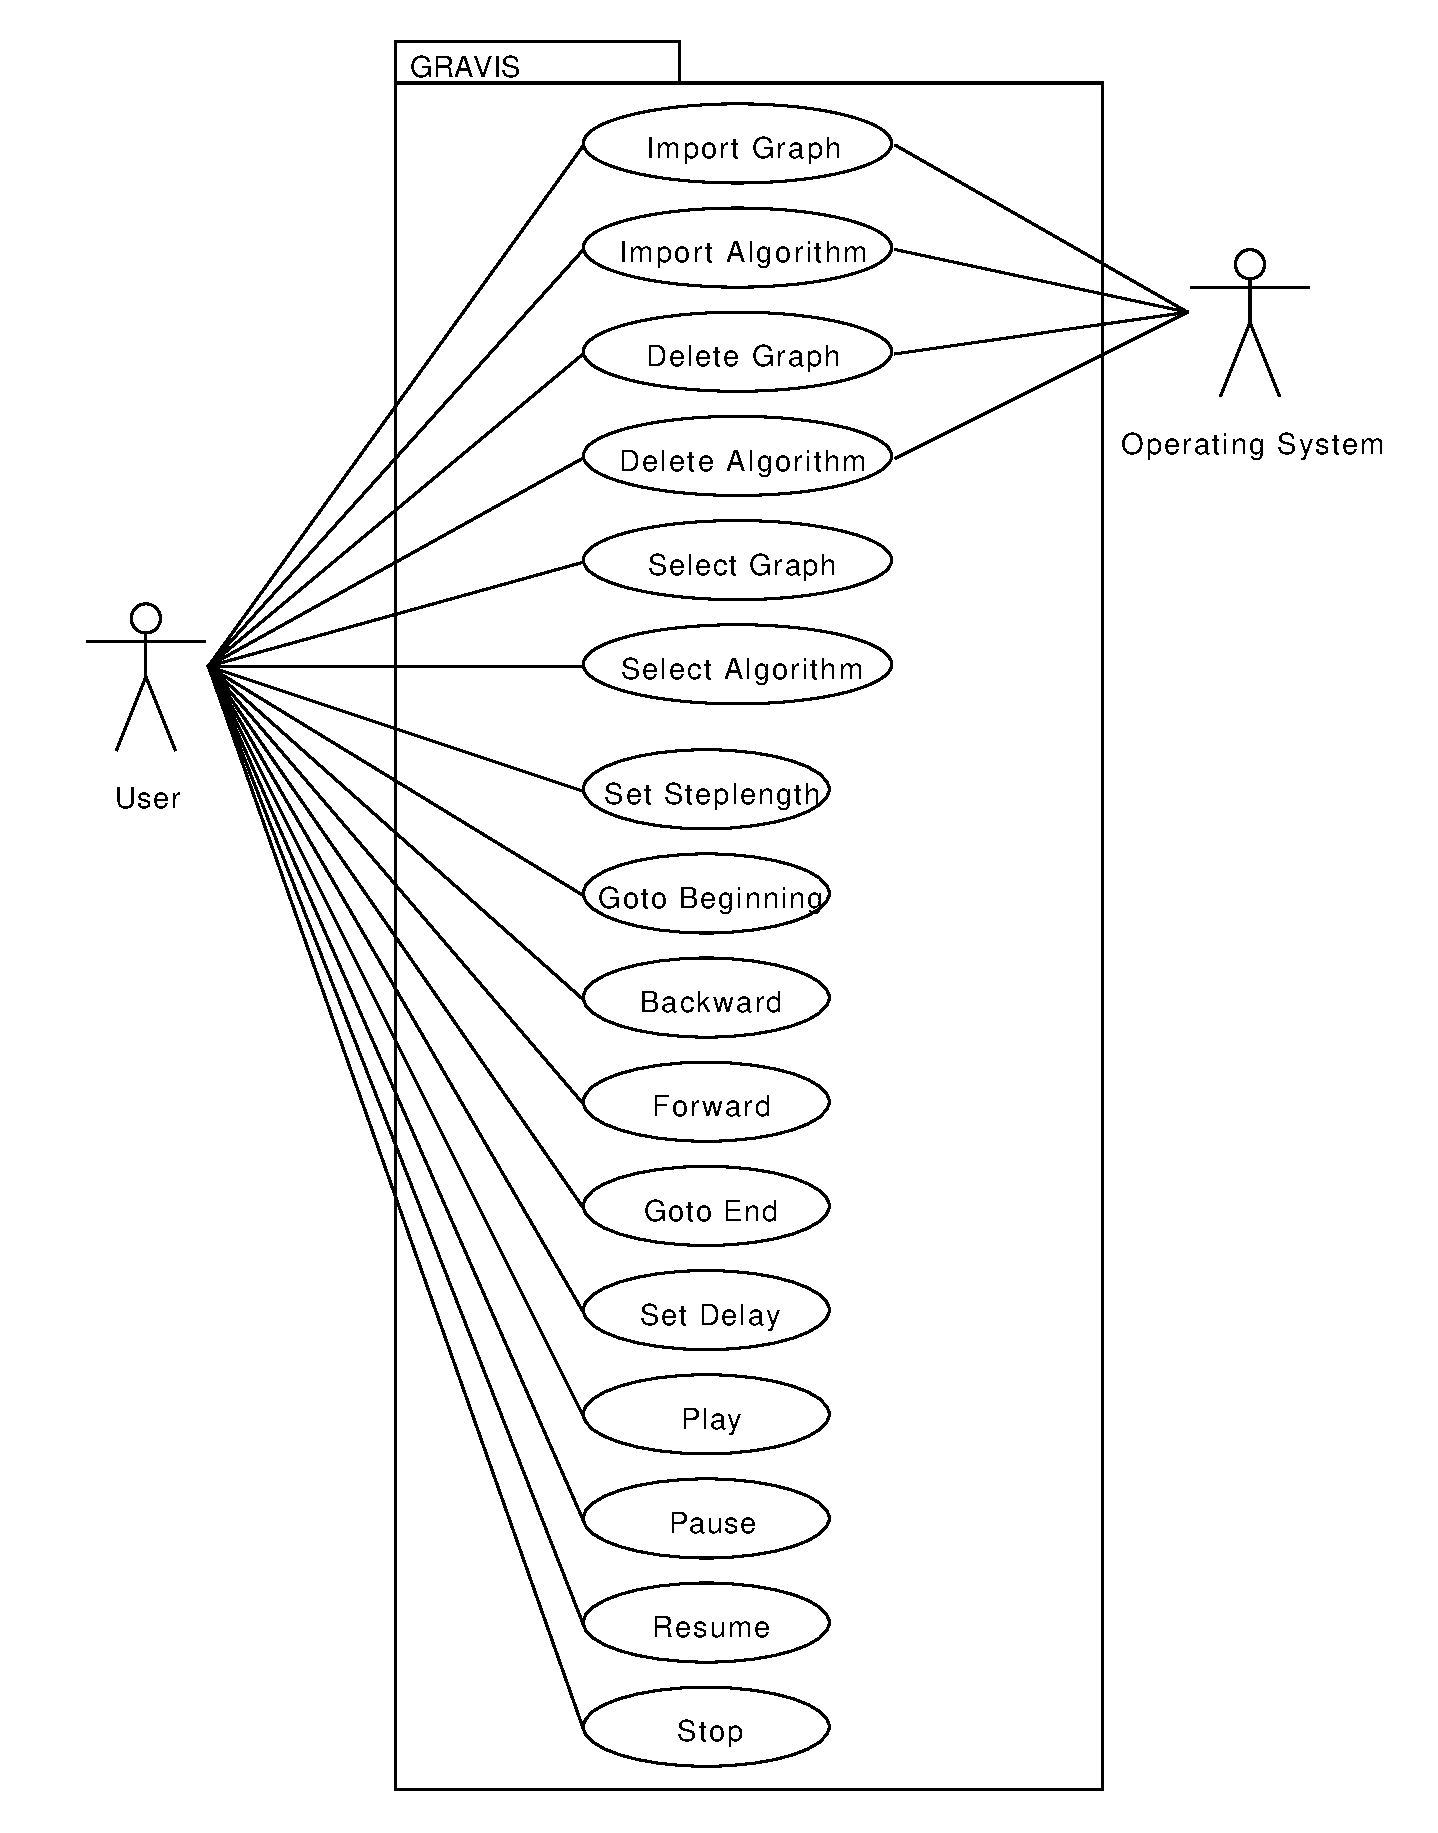
\includegraphics[scale=0.5]{diagrams/use-cases-diagram.pdf}
    \caption{Use Cases Diagram}
    \label{fig:use_cases_diagram}
\end{figure}
% 
\subsection{Use Cases in Brief Format}
\label{subsec:Use Cases in Brief Format}
% - All the use-cases of the application you discover, which have to be written in brief format;
\begin{description}
  \item[Import Graph:] Der User kann einen neuen Graphen importieren.

  (Ausgearbeitetes Format siehe Seite~\pageref{uc:Import Graph})

  \item[Import Algorithm:] Der User kann einen neuen Algorithmus importieren.

  (Ausgearbeitetes Format siehe Seite~\pageref{uc:Import Algorithm})

  \item[Delete Graph:] Der User kann einen importierten Graphen l\"oschen.

  (Ausgearbeitetes Format siehe Seite~\pageref{uc:Delete Graph})

  \item[Delete Algorithm:] Der User kann einen importierten Algorithmus l\"oschen.

  (Ausgearbeitetes Format siehe Seite~\pageref{uc:Delete Algorithm})

  \item[Select Graph:] Der User kann einen Graphen ausw\"ahlen.

  (Ausgearbeitetes Format siehe Seite~\pageref{uc:Select Graph})

  \item[Select Algorithm:] Der User kann einen Algorithmus ausw\"ahlen.

  (Ausgearbeitetes Format siehe Seite~\pageref{uc:Select Algorithm})

  \item[Set Steplength:] Der User kann f\"ur die Visualisierung die Anzahl Traversierungsschritte pro Bild einstellen.

  \item[Forward:] Der User kann in der Step-by-Step-Visualisierung ein Bild vorw\"arts gehen.

  \item[Backward:] Der User kann in der Step-by-Step-Visualisierung ein Bild r\"uckw\"arts gehen.

  \item[Goto Beginning:] Der User kann in der Step-by-Step-Visualisierung an das Ende springen.

  \item[Goto End:] Der User kann in der Step-by-Step-Visualisierung an den Anfang springen.

  \item[Set Delay:] Der User kann f\"ur die animierte Visualisierung das Zeitintervall zwischen zwei Bildern einstellen.

  \item[Play:] Der User kann die animierte Visualisierung starten.

  \item[Pause:] Der User kann die animierte Visualisierung pausieren.

  \item[Resume:] Der User kann die pausierte animierte Visualisierung wieder aktivieren.

  \item[Stop:] Der User kann die animierte Visualisierung anhalten.
\end{description}
% 
\subsection{Use Cases in Fully Dressed Format}
\label{subsec:Use Cases in Fully Dressed Format}
Die sechs UC \textit{Import Graph}, \textit{Import Algorithm}, \textit{Delete Graph}, \textit{Delete Algorithm}, \textit{Select Graph} und \textit{Select Algorithm} werden im ausgearbeiteten Format erl\"autert. F\"ur diese UC gilt:
\begin{itemize}
  \item Scope: System-wide
  \item Level: User-goal
  \item Primary Actor: User
\end{itemize}
\newpage
% 
\begin{usecase}{Import Graph}
    \preconditions{
	    \item Die Benutzerschnittstelle zur Befehlswahl ist aktiv.
	    \item Die Dateistruktur des Betriebssystems ist zug\"anglich.
	    \item Auf die zu importierende Datei sind mindestens Leserechte gesetzt.
    }
    \postconditions{
	    \item Der Parameter steht dem System zur weiteren Verarbeitung zur Verf\"ugung.
	    \item Der Parameter steht dem User in der Parameterliste zur Auswahl bereit.
            \item Der Default-Graph wurde ausgew\"ahlt.
    }
    \mainsuccess{
	    \item Der User w\"ahlt \"uber die Benutzerschnittstelle das Importieren eines Graphen (import).
	    \item Der User wird dazu aufgefordert, den Pfad und den Dateinamen einer Datei anzugeben (open) oder den Vorgang abzubrechen (abort).
	    \item Die angegebene Datei wird in die Dateistruktur des Systems kopiert (copy).
	    \item Die angegebene Datei wird durch das System auf Kompatibilit\"at gepr\"uft (load).
	    \item Der importierte Graph wird zur Graph-Parameterliste hinzugef\"ugt (add).
	    \item Der Default-Graph wird ausgew\"ahlt (select, siehe \textit{UC5 Select Graph} Seite~\pageref{uc:Select Graph}).
    }
\end{usecase}
\newpage 
% 
\begin{usecase}{Import Algorithm}
    \preconditions{
	    \item Die Benutzerschnittstelle zur Befehlswahl ist aktiv.
	    \item Die Dateistruktur des Betriebssystems ist zug\"anglich.
	    \item Auf die zu importierende Datei sind mindestens Leserechte gesetzt.
    }
    \postconditions{
	    \item Der Parameter steht dem System zur weiteren Verarbeitung zur Verf\"ugung.
	    \item Der Parameter steht dem User in der Parameterliste zur Auswahl bereit.
            \item Der Default-Graph wurde ausgew\"ahlt.
    }
    \mainsuccess{
	    \item Der User w\"ahlt \"uber die Benutzerschnittstelle das Importieren eines Algorithm (import).
	    \item Der User wird dazu aufgefordert, den Pfad und den Dateinamen einer Datei anzugeben (open) oder den Vorgang abzubrechen (abort).
	    \item Die angegebene Datei wird in die Dateistruktur des Systems kopiert (copy).
	    \item Die angegebene Datei wird durch das System auf Kompatibilit\"at gepr\"uft (load).
	    \item Der importierte Algorithmus wird zur Algorithmus-Parameterliste hinzugef\"ugt (add).
	    \item Der Default-Algorithm wird ausgew\"ahlt (select, siehe \textit{UC6 Select Algorithm} Seite~\pageref{uc:Select Algorithm}).
    }
\end{usecase}
\newpage 
% 
\begin{usecase}{Delete Graph}
    \preconditions{
	    \item Die Benutzerschnittstelle zur Befehlswahl ist aktiv.
	    \item Die Dateistruktur des Betriebssystems ist zug\"anglich.
	    \item Auf die zu l\"oschende Datei sind Schreibrechte gesetzt.
    }
    \postconditions{
	    \item Die Datei wurde aus dem System gel\"oscht.
	    \item Die Graph-Parameterliste wurde aktualisiert.
            \item Der Default-Graph wurde ausgew\"ahlt.
    }
    \mainsuccess{
	    \item Der User w\"ahlt ahlt \"uber die Benutzerschnittstelle das L\"oschen eines Graphen (delete).
	    \item Der User wird dazu aufgefordert, den Pfad und den Dateinamen der Datei anzugeben (open) oder den Vorgang abzubrechen (abort).
	    \item Der zu l\"oschende Graph wird aus der Graph-Parameterliste entfernt (remove).
	    \item Die angegebene Datei wird aus der Dateistruktur des Systems gel\"oscht (delete).
	    \item Der Default-Graph wird ausgew\"ahlt (select, siehe \textit{UC5 Select Graph} Seite~\pageref{uc:Select Graph}).
    }
\end{usecase}
\newpage 
% 
\begin{usecase}{Delete Algorithm}
    \preconditions{
	    \item Die Benutzerschnittstelle zur Befehlswahl ist aktiv.
	    \item Die Dateistruktur des Betriebssystems ist zug\"anglich.
	    \item Auf die zu l\"oschende Datei sind Schreibrechte gesetzt.
    }
    \postconditions{
	    \item Die Datei wurde aus dem System gel\"oscht.
	    \item Die Algorithm-Parameterliste wurde aktualisiert.
            \item Der Default-Graph wurde ausgew\"ahlt.
    }
    \mainsuccess{
	    \item Der User w\"ahlt ahlt \"uber die Benutzerschnittstelle das L\"oschen eines Algorithm (delete).
	    \item Der User wird dazu aufgefordert, den Pfad und den Dateinamen der Datei anzugeben (open) oder den Vorgang abzubrechen (abort).
	    \item Der zu l\"oschende Algorithm wird aus der Algorithm-Parameterliste entfernt (remove).
	    \item Die angegebene Datei wird aus der Dateistruktur des Systems gel\"oscht (delete).
	    \item Der Default-Algorithm wird ausgew\"ahlt (select, siehe \textit{UC6 Select Algorithm} Seite~\pageref{uc:Select Algorithm}).
    }
\end{usecase}
\newpage 
% 
\begin{usecase}{Select Graph}
    \precondition{
	    Die Benutzerschnittstelle zur Wahl eines Graphen ist aktiv.
    }
    \postconditions{
	    \item Der Graph wurde als ausgew\"ahlt markiert.
	    \item Der gew\"ahlte Graph steht als geladene Instanz zur weiteren Verarbeitung zur Verf\"ugung.
	    \item Der gew\"ahlte Graph ist visualisiert.
	    \item Die auf den Graphen anwendbaren Algorithmen wurden aktiv gesetzt.
	    \item Die Parameterlisten der Benutzerschnittstellen wurden aktualisiert.
    }
    \mainsuccess{
	    \item Der vormalige Graph wird im System entladen (clear).
	    \item Der gew\"ahlte Graph wird ins System geladen (load).
	    \item In der Parameterliste wird der gew\"ahlte Graph als aktuell gesetzt (set selected).
	    \item Die auf den Graphen anwendbaren Algorithm werden aktiv gesetzt (enable).
	    \item Die Parameterlisten der Benutzerschnittstellen werden aktualisiert.
	    \item Der aktuelle Graph wird im Visualizer dargestellt.
    }
\end{usecase}
\newpage 
% 
\begin{usecase}{Select Algorithm}
    \preconditions{
	    \item Die Benutzerschnittstelle zur Wahl eines Algorithm ist aktiv.
    }
    \postconditions{
	    \item Der Algorithm wurde als ausgew\"ahlt markiert (\textit{selected}).
	    \item Der gew\"ahlte Algorithm wurde als Instanz geladen.
	    \item Die Parameterliste der Benutzerschnittstelle wurde aktualisiert.
            \item Der gew\"ahlte Algorithm hat eine Traversal generiert.
	    \item Das System ist zur Visualisierung der Traversal bereit.
    }
    \mainsuccess{
	    \item In der Parameterliste wird der gew\"ahlte Algorithm als ausgew\"ahlt markiert (\textit{selected}).
	    \item Der gew\"ahlte Algorithm wird ins System geladen.
	    \item Die Parameterliste der Benutzerschnittstelle wurde aktualisiert.
	    \item Der gew\"ahlte Algorithm brechnet die Traversal.
	    \item Der User erh\"alt eine Mitteilung, dass die Berechnung der Traversal abgeschlossen ist.
	    \item Der User quittiert die Mitteilung.
	    \item Die Abspielkonsole zur Steuerung der Visualisierung wird aktiviert.
    }
\end{usecase}